\section{Introduction}

\noindent
The field at the bottom of the Eigenmath window is for entering
calculations that get evaluated right away.

\begin{center}
\begin{tikzpicture}
\node at (0,0) {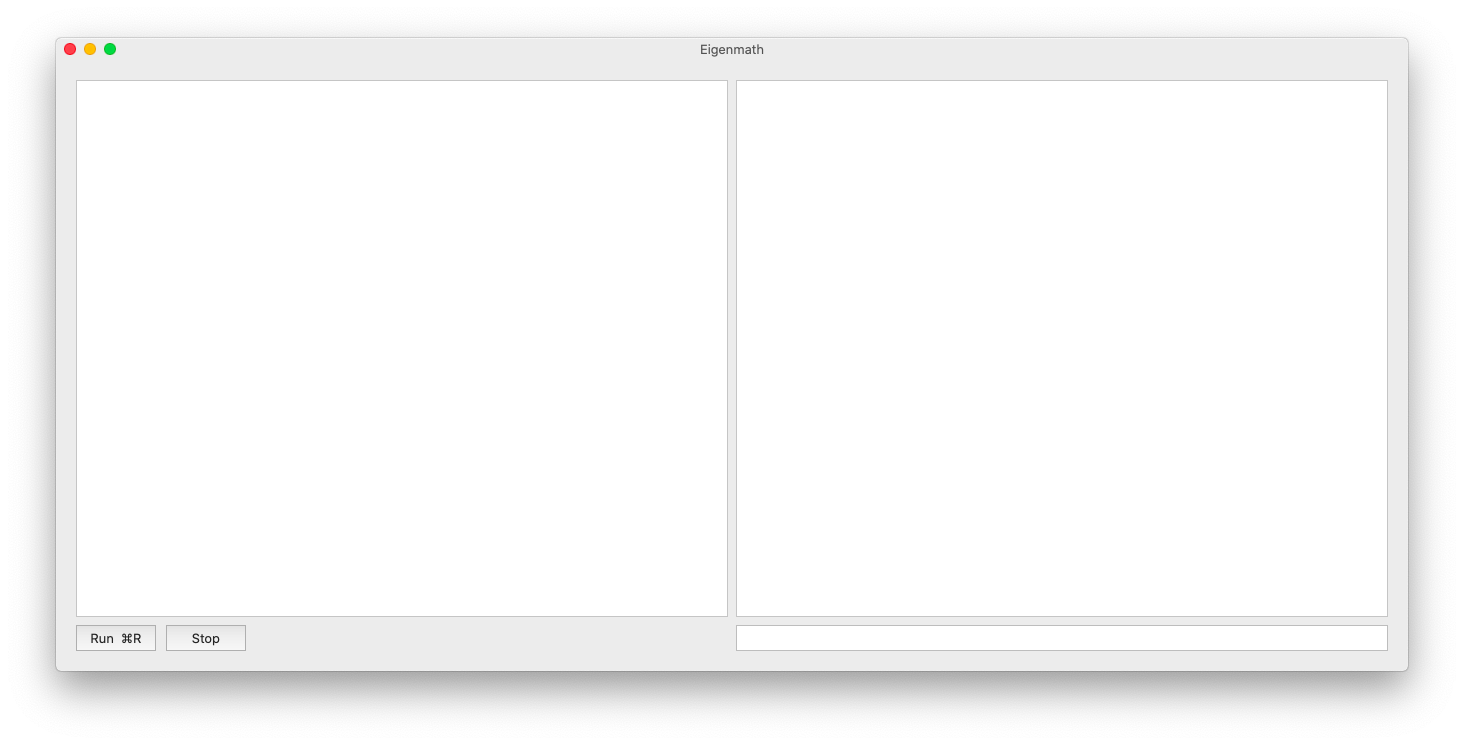
\includegraphics[scale=0.2]{face.png}};
\draw[red,thick] (2.3,-1.95) ellipse (2.5cm and 0.5cm);
\end{tikzpicture}
\end{center}

\noindent
We can use Eigenmath to check the following arithmetic from
Vladimir Nabokov's autobiography ``Speak, Memory.''

\begin{quote}
A foolish tutor had explained logarithms to me much too early, and I had
read (in a British publication, the {\it Boy's Own Paper}, I believe)
about a certain Hindu calculator who in exactly two seconds could find the
seventeenth root of, say,
352947114576027513 2301897342055866171392
(I am not sure I have got this right; anyway the root was 212).
\end{quote}

\noindent
In the field at the bottom of the Eigenmath window,
enter the following to compute $212^{17}$.

{\color{blue}
\begin{verbatim}
212^17
\end{verbatim}
}

\noindent
After pressing the return key, Eigenmath displays the following result.

\bigskip
\noindent
$3529471145760275132301897342055866171392$

\bigskip
\noindent
So Nabokov did get it right after all.
Now let us see if Eigenmath can find the
seventeenth root of this number, like the Hindu calculator could.

{\color{blue}
\begin{verbatim}
N = 212^17
N^(1/17)
\end{verbatim}
}

\noindent
Eigenmath displays the following result.

\bigskip
\noindent
$212$

\bigskip
\noindent
When a symbol is assigned a value, such as $N$ above,
no result is printed.
To see the value of a symbol, just evaluate it.

{\color{blue}
\begin{verbatim}
N
\end{verbatim}
}

\noindent
$N=3529471145760275132301897342055866171392$

\bigskip
\noindent
The previous example shows a convention that will be used throughout
this manual.
That is, the color blue indicates something that the user should type.
The computer response is shown in black.
